\section{Evaluation}
We first integrate SchemaLine into an existing visual analytics system, and then evaluate its usefulness in \annote{supporting sensemaking}{more precise of the support}.

\subsection{Application}
% Overview of INVISQUE
We integrate SchemaLine into INVISQUE -- INteractive VIsual Search and QUery Environment -- designed for interactive exploration of text documents~\cite{Wong2011}. INVISQUE organizes search results in a two-dimensional spatial canvas, with each dimension representing a customized attribute. For example, articles of \emph{publication data} can be ordered horizontally by date and vertically by citation count. Search results from a keyword are shown as a cluster of \emph{index-cards}, each representing a document with selected information such as publication title, date, keywords and authors. Figure~\ref{fig:invisque} shows a screenshot of INVISQUE.

\begin{figure}[!htb]
	\centering
	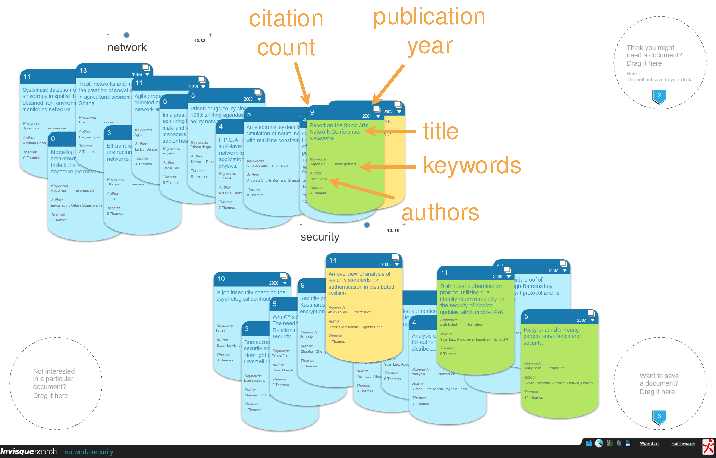
\includegraphics[width=\linewidth]{invisque}
	\caption{INVISQUE interface. It shows two sets of search results for ``network'' and ``security'' from a publication dataset. Each article is displayed as an index-card with citation count at the top left corner, publication year at the top right corner; and title, keywords and authors at the center.}
	\label{fig:invisque}
\end{figure}

% Integration
We add an \emph{annotation} feature enabling users to record their thoughts while reading documents. These annotations are important to users, thus are also displayed on the index-cards. We choose them as the input \emph{events} of the SchemaLine visualization. SchemaLine is placed at the bottom of INVISQUE.
After the user makes a note, or annotation, it is immediately added to SchemaLine as a new event. Double clicking on an event will open the document containing that note as an index-card enabling the user to quickly reexamine the original information resource.

% Attribute mapping
The \emph{temporal information} of documents, such as ``publication date'', is initially assigned to that of events, and can be changed later by users to match the correct meaning. The \emph{label} of an event is simply the content of an annotation itself. In INVISQUE, we color code search keywords that contain annotated documents, and use them as \emph{categories} for events. Because a document can be returned from different searches, it can also contain multiple categories. This mapping provides context for the annotations: what did I search for (the original keyword) and what are other related concepts (other search keywords returning the same document)? This context may help users to discover interesting patterns through their annotations later. Figure~\ref{fig:invisque-schemaline} shows a screenshot of INVISQUE with SchemaLine integrated.

\begin{figure}[!htb]
	\centering
	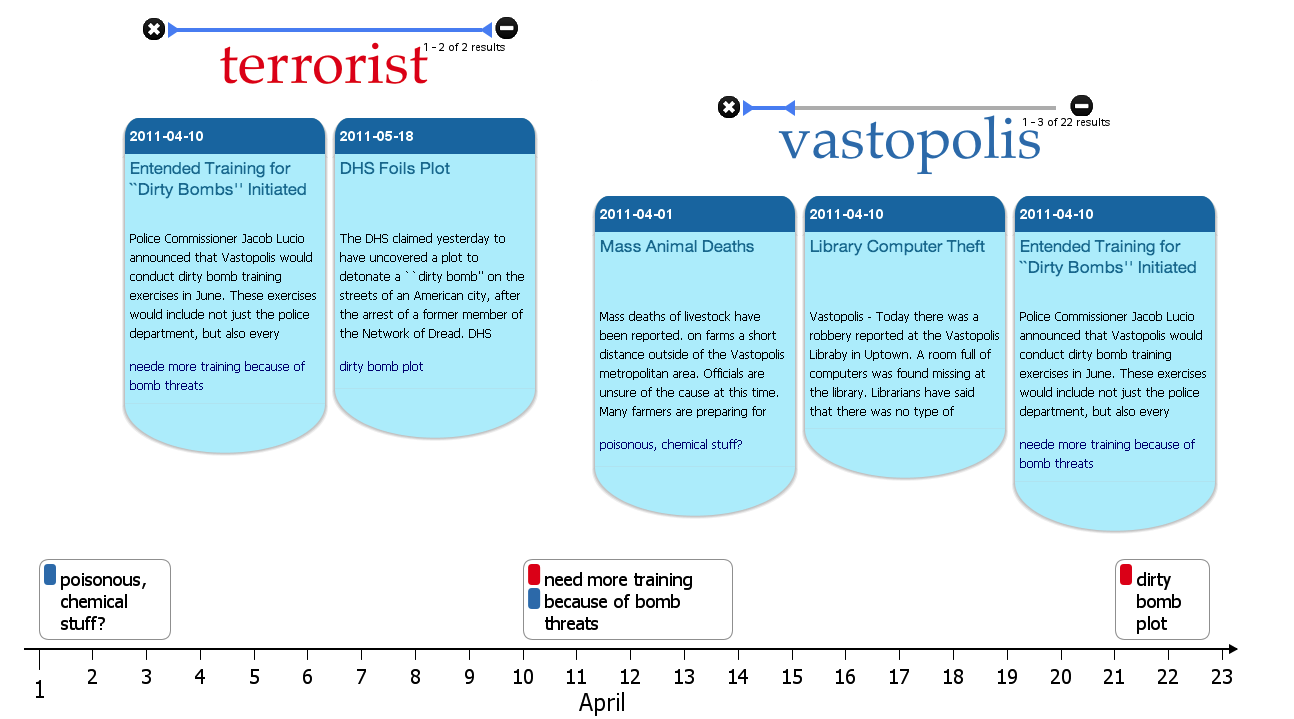
\includegraphics[width=\linewidth]{invisque-schemaline}
	\caption{INVISQUE with SchemaLine at the bottom. The timeline consists of three events, which are user taken notes. Color coded categories of events indicate keywords that were searched for.}
	\label{fig:invisque-schemaline}
\end{figure}

\subsection{Case Studies}
Evaluating the usefulness of SchemaLine in supporting sensemaking is challenging. It is categorized as \textit{evaluating visual data analysis and reasoning} -- one of seven scenarios in the information visualization empirical studies by Lam et al.~\cite{Lam2012}. Because of the difficulties of this evaluation type, such as the fluidity and various approaches used by analysts and the quantification of the analysis results, evaluations are typically case studies with realistic datasets and domain experts as participants.

We used the task from Mini Challenge 3 of the VAST Challenge 2011, which requires the participants to identify any potential criminal activities from the given dataset. INVISQUE with SchemaLine integrated was used in the study. This dataset was chosen because the solution was provided and well-tested by the community. The original dataset contains four thousand news reports, many of which are over 500 words long. A pilot study showed that it was difficult for the participant to find any answers even after trying for a long time. The reason could be INVISQUE does not support text-mining features such as entity extraction, which is crucial in analyzing a large document collection. The goal of the evaluation is to assess how SchemaLine can support INVISQUE in sensemaking, not to assess INVISQUE itself so, in the actual study, we reduced the dataset to contain only 36 documents that were manually added into the dataset as part of the ground truth so that participants could complete the task with reasonable time and effort but without affecting the goal of the evaluation. Five criminal activities are embedded into those documents including food poisoning (13 documents), hacking (3), dirty bomb (6), arms trafficking (4), and money laundering (3) together with 7 isolated cases, which are not considered as correct solutions.

SchemaLine is designed for general-purpose usage. We tried to recruit participants with varying backgrounds, and conducted three case studies with a graduate student in visual analytics (surrogate for visualization expert, \textbf{P1}), a graduate student in law (surrogate for domain expert, \textbf{P2}), and a graduate student in networking (neutral background participant \textbf{P3}). A 10-minute-training session was given before an one-hour main task to help participants become familiar with the basic functions of INVISQUE and the set of interactions that SchemaLine offers to group relevant notes. After finishing their analyses, participants reported the criminal activities they had discovered, together with the supporting evidence. The main methods of these case studies were observations and interviews, which focused on how SchemaLine facilitates the participant in finding the answers in the context of the five sensemaking activities in the Data-Frame model it is designed to support.

%To focus participants' attention on the SchemaLine visualization, we divided the study into two sessions: both used the same visual analytics system (INVISQUE), but the first session did not have the SchemaLine and the second session did. Each session lasted 45 minutes. The task is the same for both sessions, but they did not share any news reports. The challenge solution contains one imminent threat and five other false leads. We considered all six scenarios to be valid answers and divided them equally between the two sessions; the rest of the news reports were distributed between the two sessions so that each had 30 in total.

%We recruited two participants, who were both postgraduate students conducting sensemaking-related research. A 10-minute-training was given before the actual task to help participants get familiar with the basic functions of the INVISQUE environment. During the actual task, a think-aloud protocol was used, and participants' screen and audio were captured for the entire duration. Participants had the option to take notes with paper/pen or word processing software such as Microsoft Word, besides what is available in INVISQUE. At the end of each session, participants reported the criminal activities they identified with all news reports that lead them to the findings. A semi-structured interview was conducted once both sessions finished. 

%\textbf{P1} and \textbf{P3} started by searching keywords related to criminal activities such as ``terrorism'' or ``dirty bomb''. \textbf{P2} took an overview step before searching. He quickly look at all 36 document titles to have a glimpse of the dataset as well as detect potential search keywords. Using different strategies; however, they all took notes when reading. \textbf{P1} thought that storing notes on the timeline besides rendering them on the index-cards was useful because ``now I can minimize the search result cluster to save display space but not worry of losing my notes''.
% \vspace{-4mm}
\subsubsection{Case Study 1 -- Visual Analytics Graduate Student}
Participant \textbf{P1} began searching for ``bomb'', read, took notes and continued searching for a more detailed keyword ``dirty bomb''. He used drag-and-drop interaction to link his three notes of ``dirty bomb'' documents together (\textit{construct a new frame}). Then, he searched for ``Network of Dread'', which was mentioned in one document as the author of the dirty bomb attack. He took notes on the new returned document and dropped it onto the color stripe of dirty bomb (\textit{elaborate a frame}). While investigating, he encountered an article about a man carrying a frozen turkey having wires coming out it, which was suspected as a bomb. At first, he dropped the ``turkey bomb'' note onto the ``dirty bomb'' stripe. Then, he wondered ``Is it a real bomb?''. After thinking for a while, he removed it out of the stripe (\textit{preserve a frame}), which was a correct decision when checking against the solution.

\begin{figure*}[ht]
\centering
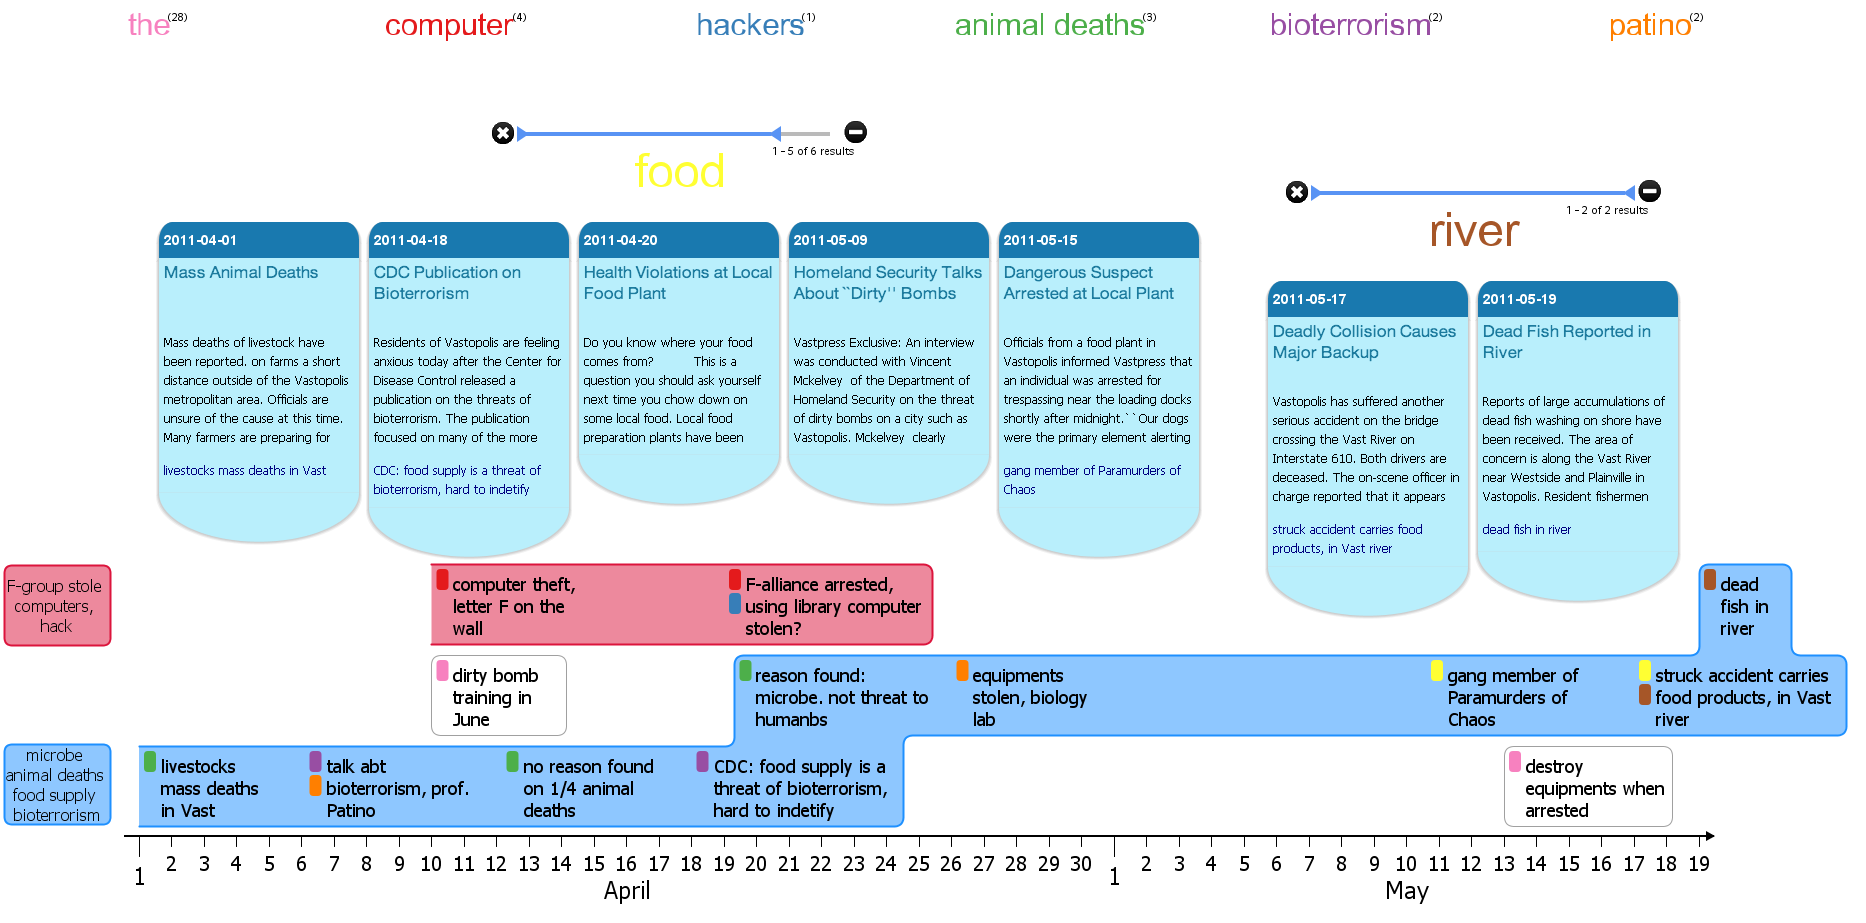
\includegraphics[width=\linewidth]{evaluation}
\caption{A reproduced image from the video record of participant \textbf{P2} when he reported his findings. Top: a trail of his keyword searches, collapsed after being read. Middle: search results in index-card metaphor. Bottom: two schemata containing notes as supporting evidence of criminal activities he found.}
\label{fig:evaluation}
\end{figure*}

% \vspace{-4mm}
\subsubsection{Case Study 2 -- Law Graduate Student}
Participant \textbf{P2} took an overview step before searching. He quickly looked at all 36 document titles to have a glimpse of the dataset as well as to detect potential search keywords. He began searching ``animal deaths'', read, took notes and grouped them together (\textit{construct a new frame}). He was happy with the evidence he found for that crime and switched to read another interesting article ``Library Computer Left'' he came across. From that, he searched for several related terms such as ``computer'' and ``hackers''. He figured out that a group called ``F-alliance'' stole computers from the library and attempted to hack a bank. He dropped the ``computer stolen'' note on top of the ``bank hacking'' note to form a new explanation for the case (\textit{construct a new frame}). He found another article related to hacking but he said ``I won't drop it to this group because it's just an announcement from the government about potential threats'' (\textit{preserve a frame}). During further investigation, he created another group of notes related to ``bioterrorism'' and ``Prof. Patino''. Then, when figuring out that the reason of the mass deaths is a spore-forming microbe, which is also mentioned in Prof. Patino's talk, he dragged the new group and dropped it onto the ``animal deaths'' group to combine all notes together because they are related (\textit{merge frames}). Observing the event orders in the new group on the timeline, he said ``The equipment of Patino was stolen after the animal deaths report, so they couldn't be used in that case. This is the group of potential threat in using bioterrorism'' (\textit{elaborate a frame}). Fig.~\ref{fig:evaluation} shows the computer screen of \textbf{P2} when he reported his findings.

% \vspace{-4mm}
\subsubsection{Case Study 3 -- Computer Network Graduate Student}
Participant \textbf{P3} searched for a few keywords related to criminal activities before investigating the search results such as ``bomb'', ``terrorism'', ``money'' and ``hack''. In a similar fashion to other participants he took notes when reading, and grouped related notes together by dragging one note and dropping it on top of another note (\textit{construct a new frame}). After finding a crime about money laundering, he read articles from ``terrorism'' search results. Then, he followed the article content to search for relevant information such as ``Paramurderers of Chaos'' -- a terrorist group. During further investigation, similar to \textbf{P2}, he also combined two groups of notes -- ``Paramurderers of Chaos'' and ``food supply'', together when discovering evidence linking the two groups (\textit{merge frames}). When representing his findings, he shared that SchemaLine prompted him to look for missing information. ``I noticed the gap between these two events [pointing to the timeline]; then I knew I probably missed something there'' (\textit{question a frame}).

%\paragraph*{Reframing}
%No participants needed to compare alternative frames. The reason could be that all criminal activities embedded into the dataset are sufficiently different to not be confused: food poisoning, hacking, dirty bomb, arms trafficking, and money laundering.
% \vspace{-4mm}
\subsubsection{Participant Results and Discussion:}
\textbf{P1} found the ``dirty bomb'' attack with 4/6 pieces of evidence. \textbf{P2} found the ``hacking'' case with 2/3 pieces of evidence, and the ``food poisoning'' case with 9/13 pieces of evidence. \textbf{P3} also found the ``food poisoning'' case with 6/13 pieces of evidence, and a perfect 3/3 pieces of evidence in the ``money laundering'' case. \textbf{P1} took many notes in documents related to the ``food poisoning'' case; however he could not link them together because ``I'm not familiar with bio-attack so I couldn't think of it as a threat''. All participants extensively used SchemaLine to group related notes with different types of relationship: a group of ``bioterrorism'' articles, a group of more specific criminal activity like ``dirty bomb'' or ``money laundering'', a group of people like ``Paramurderers of Chaos'', and a group of a specific person like ``Prof. Patino''. Another benefit of using SchemaLine is that all participants are very confident when presenting their analyses. \textbf{P3} even opened the original document (double-clicking on the note) several times to highlight the relevant text when reporting to the observer to show his strong evidence. \textbf{P1} had a scenario about \textit{airport attack} with only two pieces of evidence. He said that he was not sure about that and he did not think it was correct. Indeed, it was not mentioned in the solution. It proved that the participants justified evidence a lot to provide a reliable answer when using SchemaLine.

In summary, all participants liked the feature of automatically adding notes to the timeline so that they did not need to remember the notes. \textbf{P1} thought that he would have problem if the system did not support that: ``I can remember what happened but it was difficult to remember when it happened''. They found that it was helpful to build a scenario with SchemaLine because the information is organized chronologically, which is the order when events actually happened. \textbf{P2} shared that he read the news about the robbery at Vastopolis university and the Prof. Patino's talk about bioterrorism. He did not have any insight at that time. However, when looking at his two notes on the timeline, he realized that the order of the two events was the other way around. Then, he thought that Prof. Patino's description of extremely expensive equipment in his lab could be the rationale of the robbery. All participants commented that the interactions to edit frames are very intuitive. \textbf{P1} even said ``I think I don't even need training and still can figure out how it works''. \textbf{P3} liked the transition effect when adding or removing notes because ``it helped me to understand what is going on''. These case studies showed the usefulness of SchemaLine in supporting sensemaking as well as the intuitiveness and effectiveness of SchemaLine's interactions in performing those sensemaking activities. 

% The application prototype can be found at \url{http://www.youtube.com/watch?v=zxF-TEF11F8}.
% Regarding note taking, both participants commented that writing notes directly on an index card was useful because it linked the notes with the news report. However, during the session without the SchemaLine, it became difficult as the number of search results increased. Participant \textbf{P1} said: ``I could minimize search result cluster to make more space for new searches, but I do not really like this because I cannot see the notes in such clusters and will forget which reports already have notes.'' He expressed the need of ``a more structural way to organize annotated documents and save display space''. After the session with the SchemaLine, both participants commented that organizing notes using the Story was a nice feature because they would not lose what they wrote down. \textbf{P1}: ``now I can minimize the search result cluster to save display space but not worry about losing my notes''. 

% Once there were several notes, both participants started to examine the relationships among the events they identified. In the first session (no SchemaLine), both participants did this by grouping reports that they thought were related: they dragged each report index card out from its search result cluster and moved all of them to the same empty space to form a new group (a feature in INVISQUE). In the second session, both participants used the SchemaLines to group their notes. This is also how both participants reported their findings at the end of each session.

% Both participants liked the feature of automatically adding notes to the timeline. They both found it easier to build a scenario with the SchemaLine because the information is more organized. They appreciated the organization of notes by event time because the chronological order made it easier to piece together a scenario. Participant \textbf{P2} mentioned that the SchemaLine visualization prompted him to look for missing information. ``I noticed the gap between these two events (on the SchemaLine); then I knew I probably missed something there''. 

% When reporting their findings, Participant \textbf{P1} had two reports in the wrong order in the first session. He later explained that ``I can remember what happened but it was difficult to remember when it happened''. In the second session, he was pleased with the ordering feature of the SchemaLine and did not make any similar mistake. Both participants were more confident about their answers in the second session and believed that they found more correct answers than in the first session. This was true after checking against the solution. The answers were also more complete in the second session, i.e., it was less likely that there were missing reports in the answer. The ability to see the gaps in the timeline may have prompted them to look for missing information. The opposite is true for the first session, and Participant \textbf{P1} created a implausible scenario that he could not explain himself during the reporting. 

% Both participants commented that the SchemaLine features for scheme creation and editing are very intuitive: ``I think I don't even need training and still can figure out how it works''. This is also reflected in the observation that they made more refinements to their answers with the SchemaLine than in the first session. They both liked the transition effect when adding/removing notes because ``it helped me to understand what is going on''. Participant \textbf{P2} mentioned that the grouping feature in SchemaLine helped him to organize events to build a story. However, very often, he could not decide in which group the news report should go: ``I felt this [report] was relevant, but can't decide which group yet. I just wanted to put it aside to read it later''.